\chapter{GL-117 Aerodynamics}
\label{chap:aerodynamics}

This chapter gives a brief introduction on all the physics
a pilot has to consider when flying an aircraft.

\section{The four forces}
\label{sec:forces}

During flight the four forces acting on an aircraft are \texttt{lift},
\texttt{drag}, \texttt{thrust}, and \texttt{weight}, see fig \ref{fig:forces}.

\texttt{Lift} is the upward force created by the airflow as it
passes over the wings.
In straight, unaccelerated flight, the lift compensates the
\texttt{weight force} and therefore, the aircraft does not climb or dive.
The lifting force depends on the speed: low speed will cause the
airplane to dive, at high speed it will even climb.
Always consider the lift vector. If you fly a roll, the lift will not
oppose the weight any more and thus, you will lose height.

\texttt{Drag} is the retarding force that limits the aircraft's speed.
There are many factors effecting drag, but one main cause
is simply the airplane's structure that protrudes into the wind.

\texttt{Thrust} is the forward force provided by the engines.

However \emph{GL-117} uses a simplified aerodynamics model making
it much easier to handle the aircraft. The four forces are
simulated in a very easy way and not very realistic. \emph{GL-117}
does not claim to be a training simulator, but aims to provide
as much action as possible.

\begin{figure}
\begin{center}
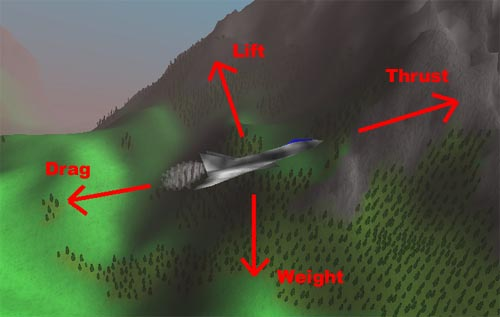
\includegraphics[width=10cm]{forces.jpg}
\caption{The four forces}
\label{fig:forces}
\end{center}
\end{figure}



\section{Three rotation axes}
\label{sec:axis}

All maneuvering takes place around three axes of rotation.
One way to define these axes is a carthesian coordinate system
with an x axis from left to right,
a y-axis from top to bottom, and a z-axis from near to far.
Imagine a flat landscape resembling the x-z plane.
Your viewing angle within this plane is called the \texttt{heading},
whereas an orthogonal angle is called the \texttt{elevation}.
Just look at figure \ref{fig:heading}.

But we can also define three axis of rotation referring to our fighter.
They are known as the \texttt{longitudinal axis}, \texttt{lateral axis},
and \texttt{vertical axis}.
Imagine a coordinate system with the origin at your fighter's center of gravity.
The center of gravity is the theoretical point where the entire weight
of the aircraft is considered to be concentrated.

The \texttt{lateral axis} is an imaginary axis protruding through the side
of the aircraft. A rotation around this axis is known as pitching.
This pitch movement is produced by the elevators and
will affect your heading and elevation.

The \texttt{longitudinal axis} is an imaginary axis protruding through
the nose of the aircraft.
A rotation around this axis is known as a roll.
This roll movement is produced by the ailerons.
Consider that a roll will not change your heading.

The \texttt{vertical axis} is an imaginary axis protruding through the top and
bottom
of the aircraft. A rotation around this axis is know as yawing.
This yaw movement is produced by the rudder.

Now, look at fig \ref{fig:fly}.
The blue arrows show the elevator's effect: your fighter will
either move up and left or it will drop down to the right
(the lateral axis).
Using the rudder will move the fighter slightly towards the green arrows
(the vertical axis).

\begin{figure}
\begin{tabular}{p{7.2cm}p{7.2cm}}
\begin{center}
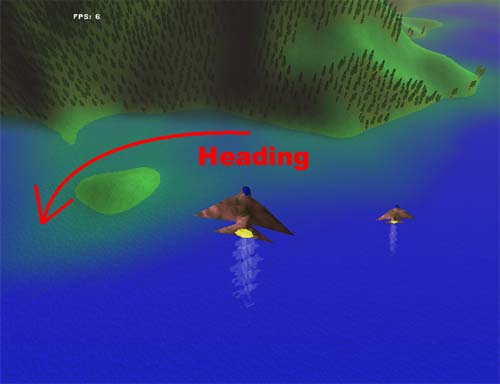
\includegraphics[width=7.2cm,height=6cm]{heading.jpg}
\label{fig:heading}
\end{center} &
\begin{center}
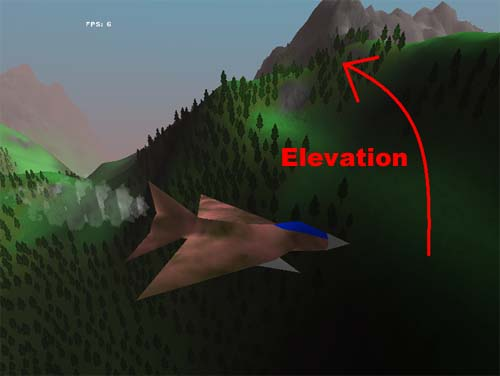
\includegraphics[width=7.2cm,height=6cm]{elevation.jpg}
\label{fig:elevation}
\end{center}\\
\begin{center}
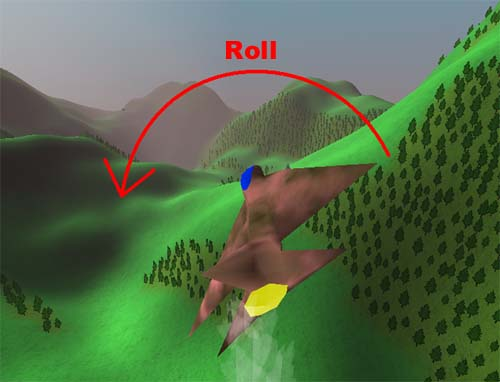
\includegraphics[width=7.2cm,height=6cm]{roll.jpg}
\label{fig:roll}
\end{center} &
\begin{center}
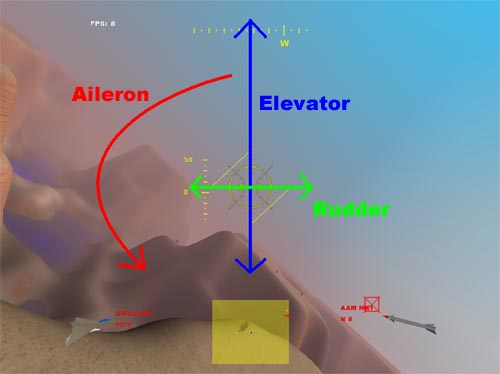
\includegraphics[width=7.2cm,height=6cm]{fly.jpg}
\label{fig:fly}\\
\end{center}
\end{tabular}
\caption{The three axes of rotation}
\end{figure}
